% Chapter Template

\chapter{Architecture} % Main chapter title

\label{ch:arch} % Change X to a consecutive number; for referencing this chapter elsewhere, use \ref{ChapterX}

\lhead{Chapter \ref{ch:arch}. \emph{Architecture}} % Change X to a consecutive number; this is for the header on each page - perhaps a shortened title

%----------------------------------------------------------------------------------------
%	INTRO TEXT
%----------------------------------------------------------------------------------------

The outcome of this thesis project is \pname, a music player application that accepts English utterances as commands, adapts to utterances it has never been exposed to, and learns from them by possibly interacting with the user, thus expanding its initial knowledge of the language. The application has been written in Python 2.7, and consists of a client application for the existing OpenTDM dialogue management library. Such a library supports basic dialogue management based on the Information State Update approach, but has no support for grounding or flexible understanding of unknown sentences. Therefore, TDM has been extended with the Language Unit module, that introduces these capabilities.
% TODO: mention interpretation and generation models with ref to Staffan A.9

Section \ref{ch:arch:client} describes the \pname client, Section \ref{ch:arch:TDM} describes the OpenTDM library, and Section \ref{ch:arch:LU} describes the Language Unit module.


%----------------------------------------------------------------------------------------
%	CLIENT
%----------------------------------------------------------------------------------------

\section{The Client Application} \label{ch:arch:client}
\pname is a client application for OpenTDM, a dialogue management library based on the work by \cite{Larsson02issue-baseddialogue}. An OpenTDM application can be seen as a container for domain-specific \textbf{parameters} for the dialogue manager. These parameters consist of:
\begin{itemize}
\item A \textbf{device} class, containing variables and methods that directly control the actions of the application. The \textit{device} file of a music player application will contain, for instance, variables holding the current playlist, or the current volume level, and methods to play/stop the music, lookup for a song and so forth.
\item An \textbf{ontology}, whose main purpose is to define predicates and actions that will be used at dialogue management level. In the case of \pname, an example of predicate is \texttt{current\_song(X)}, that identifies the song currently being played (note that such a predicate must be mirrored in the device file as a variable\footnote{The actual implementation consists of an inner \texttt{current\_song} class of the device class, which access the proper, private, variable of the device file through a \texttt{perform()} method. The reasons that led to such an implementative choice were not made known by the authors of OpenTDM.}); an example of action is \texttt{increase\_volume} that, intuitively, identifies the action of increasing the volume (actions are mirrored as well in the device class, in the same way predicates are).
\item A \textbf{domain} file, whose main purpose is to contain the list of plans that will control the dialogue episodes. For instance, the TOP plan of an application is to find out what the user wants to do. Another example of a plan in \pname is the \texttt{increase\_volume} plan: step 1 of the plan is to ask the user for how much the volume should be increased, step 2 is to perform the actual action through the device.

Figure \ref{ch:arch:client:increaseplan} shows the plan item, as it is defined in the application domain: we notice that the \texttt{plan} section is a list of two elements, a \texttt{findout()} function, that will ask the user for the amount of volume to increase, and a \texttt{dev\_perform()} function, that will fire the volume increasing method in the device.
\begin{figure}
\begin{Verbatim}[frame=single]
{
  "goal": "increase_volume",
  "plan": [
              "findout(?X.volume_to_increase(X))",
              "dev_perform(
			   IncreaseVolume,
			   MplayDevice,
			   {postconfirm=True}
			  )"
	   ],
  "postconds": ["done(IncreaseVolume)"]
}
\end{Verbatim}
\caption{The \texttt{increase\_volume} plan of \pname.}
\label{ch:arch:client:increaseplan}
\end{figure}
\item A \textbf{grammar} implemented using the Grammatical Framework\footnote{http://www.grammaticalframework.org/} \citep{citeulike:346448}. This part will not be discussed, since, as it is explained in Section \ref{ch:arch:LU}, the Grammatical Framework in OpenTDM has been replaced with a specifically created module called Language Unit (LU). However, the purpose of the two modules is the same, and covers what in Section \ref{ch:introduction:arch} we called language understanding and response generation. That is, mapping natural language user utterances to their formal representations and vice versa.

In the example of Figure \ref{ch:arch:client:increaseplan}, a language understanding use of the Language Unit is to take, for instance, the input sentence ``Increase the volume" and turn it into a \texttt{request(increase\_volume)} user move, that will be used to load the proper plan from the domain. A response generation use of the LU will be, for instance, to take the \texttt{ask(?X.volume\_to\_increase(X))} system move (that will be produced by the \texttt{findout()} part of the plan), and turn into a sentence like ``By how much you want the volume to be increased?".
\end{itemize}

The dialogue management logic is left to OpenTDM, that will be discussed in the next section.


%----------------------------------------------------------------------------------------
%	TDM
%----------------------------------------------------------------------------------------

\section{OpenTDM} \label{ch:arch:TDM}
OpenTDM is a \textbf{dialogue management library} developed and maintained by Talkmatic\footnote{http://talkamatic.se/} based on the Information State Update framework (see \ref{ch:rw:ds:isu}). OpenTDM is a Python 2.7 port of the TRINDI Dialogue Move Engine Toolkit \citep{Larsson:2000:ISD:973935.973943}, that was originally implemented in Prolog.

The purpose of OpenTDM is to keep track of the Information State (IS), updating it on new user utterances, and planning the system moves accordingly. This is done by applying the standard ISU rules and policies \citep{Larsson02issue-baseddialogue} to the resources defined by the application (ontology, domain, device and language). Appendix \ref{a:isu} presents an example of how SVPlay's information state changes during an interaction with the user.

It is worth to note that OpenTDM is not yet available to the public, and comes with \textbf{no documentation}. This has significantly limited us in the design of the solution, preventing us from both implementing elaborated extensions of it (e.g.\ more complex learning interactions than the ones described in Chapter \ref{ch:interaction}), and respecting the software architecture best practicses, as many of the OpenTDM extensions that we have implemented rely consistently on hacks and temporary workarounds.

%----------------------------------------------------------------------------------------
%	LU
%----------------------------------------------------------------------------------------
\section{The Language Unit} \label{ch:arch:LU}
The Language Unit (LU) is a Python library that has been specifically created to support \pname's utterances understanding ability, serving as a drop-in replacement for the Grammatical Framework, that is used in the main OpenTDM branch. The purpose of this library is to perform the classification task as it has been defined so far, that is, assigning every input sentence to its correct meaning label.

\subsection{Language}
The \texttt{Language} class is the main class of LU, its purpose is to model a natural language under the following \textbf{abstraction}: a Language is defined by a finite set of Meanings (labels); a Meaning is defined by a finite set of Sentences expressing that Meaning. As an example, the \pname language consists of a number of meanings, each of them defining an action for the application to perform; one of these meanings can be the one to pause the current song; this meaning will be realized by a number of English sentences, like ``Pause the song", ``Suspend the music", or ``Pause the current track". For the purpose of language understanding, a Sentence can be brougth down to any of its (linguistic or non-linguistic) constituents called Chunks or Phrases. A chunk is formed by one or more Words.

The following are the main capabilities implemented in the Language class:
\begin{itemize}
	\item \textbf{Load} and \textbf{save} languages. Each OpenTDM application must define a \texttt{language/} folder where the language is stored, in the form of a \texttt{.l} file. Such a file is just a dump of all the meanings and their example sentences. Since the language  can evolve through learning, applications' language files are updated every time the application is run and dialogue interactions are performed. This update consists of adding new examples to meanings (unknown sentences from the user that have been understood with a good degree of confidence) and updating the usage count of the known examples that have been processed during the interaction with the user.
	\item \textbf{Learn} a sentence. When a new labeled example (a sentence with its meaning label) is provided, the knowledge of the language is extended. This is done adding the new sentence to the list of sentences realizing that meaning, and drawing statistics (e.g. the frequency of a certain word/phrase in the given meaning) to improve the model of the meaning. Note that, when a language is loaded for the first time, every sentence in it is run through the learning procedure to initialize the statistics.
	\item \textbf{Understand} an input sentence. The core task of the Language Unit is to associate an input sentence with its correct meaning. While this operation is trivial when the input sentence is already present in the language, it becomes hard for unknown examples. In this latter case the LU computes a score for the sentence against each of the meanings that are present in the language; the meaning that achieves the best score is given as an output, along with the score itself, representing the degree of confidence for the output to be correct. The way sentences are scored is presented in the next section.
\end{itemize}

\subsection{Scores} \label{ch:arch:LU:scores}
The way the Language Unit understands a sentence is based on a number of nested comparisons, resulting into as many comparison scores. A \textbf{score} is a linear combination of separate features. The top-level task is to score the sentence against every meaning in the application database; for each of them a \textbf{Meaning Score} (see \ref{ch:arch:LU:scores:meaning}) is computed, representing how likely the input sentence is to be a realization of that meaning. This score is based on the similarity of the input sentence with the known sentences realizing the meaning; the \textbf{Sentence Score} (see \ref{ch:arch:LU:scores:sentence}) represents the similarity between two sentences. This score is based on how similar the (linguistic or non-linguistic) components of the two sentences are; any sub-string of a sentence is called Chunk, and the \textbf{Chunk Score} (see \ref{ch:arch:LU:scores:chunk}) represents the similarity between two chunks. The Chunk Score is based on the similarity of the words contained in the two chunks; the \textbf{Word Score} (see \ref{ch:arch:LU:scores:word}) represents the similarity between two words.

\subsubsection{The \texttt{Score} Data Structure}
Scores in the application are modeled by the \textbf{\texttt{Score} class} (\texttt{lu/score/\_\_init\_\_.py}). A \texttt{Score} object defines the following \textbf{fields}:
\begin{itemize}
	\item \texttt{Score.features}, an array of N features that are used to form the final score. A feature is represented as a floating-point (\texttt{float}) number.
	\item \texttt{Score.weights}, an array of N weights that are used in the linear combination of features to form the final score. A weight is also represented as a floating-point (\texttt{float}) number. Weights are equally distributed by default, but they can be overridden with custom values. To this respect, an ideal scenario would be the one in which \textbf{optimal weights} for the features are determined with machine learning (\emph{meta-model learning}), as it will be described in Chapter \ref{ch:conclusions}. % TODO: REFINE CITATION, maybe also cite Watson
\end{itemize}
Implementation-wise, for the sake of efficiency, the Python \texttt{array} module\footnote{http://docs.python.org/2/library/array.html} is used instead of traditional lists and dictionaries. Such a module defines ``an object type which can compactly represent an array of basic values", directly based on their original C implementation. The acces to the elements of an \texttt{array} is positional. For this reason any instantiation of \texttt{Score} is recommended to define proper \textbf{constants} to access the single features.

The \texttt{Score} class also defines the following \textbf{methods}:
\begin{itemize}
	\item \texttt{Score.set\_feature(i, value)}, sets \texttt{value} as the value of the the $i$-th feature.
	\item \texttt{Score.get\_feature(i)}, returns the value of the the $i$-th feature.
	\item \texttt{Score.get\_score()}, returns the final score, as the weighted average of the features:
	\begin{displaymath}
		\sigma=\sum\limits_{i=1}^Nw_if_i
	\end{displaymath}
	Where $\sigma$ is the final score, $N$ is the total number of features, $f_i$ is the $i$-th feature and $w_i$ is the weight of the $i$-th feature.
\end{itemize}

Parallel to its class definition, any subclass of score must define a list $h = \{h_1, ..., h_N\}$ of procedures, called \textbf{hooks}, that compute the single features of the score, and a \textbf{factory} method, which runs the two elements to be compared through the feature hooks, fills a score object with the results and returns it. As an example, let's consider a fictional Word Score class, that scores the similarity of two English words, and that has only one feature, being the edit distance between the two words. In this case the hooks list will contain only one element ($h=\{h_1\}$), which is a pointer to a procedure \texttt{c\_edit\_distance(word\_from, word\_to)}, that returns the edit distance between two input words. The factory function \texttt{get\_score(word\_from, word\_to)}\footnote{Not to be confused with the \texttt{Score.get\_score() method.}} will instanciate an empty score object, and will assign the result of the computation of every feature hook $h_i$ to the corresponding feature $f_i$; therefore, the only feature of the score, representing the edit distance, will be filled with the result of \texttt{c\_edit\_distance}.

The following sections describe how the \texttt{Score} class is \textbf{extended} to model the different levels of scores that were introduced above.

\subsubsection{Meaning Score} \label{ch:arch:LU:scores:meaning}
A Meaning Score $\sigma_M(s,m)$ represents the likelihood of the sentence $s$ to be a realization of the meaning $m$. It is represented in the application by the \texttt{MeaningScore} class (\texttt{lu/score/meaning.py}), which is a subclass of \texttt{Score}. Such a class defines the following \textbf{three features}:
\begin{itemize}
	\item \texttt{MeaningScore.MAX\_SSCORE} - The best similarity score between the input sentence and one of the sentences that realize the meaning.
	\begin{displaymath}
		\sigma_{M,\text{MAX\_SCORE}}(s,m) = \max{\sigma_S(s,s_i)}
	\end{displaymath}
	Where $\sigma_{M,\text{MAX\_SCORE}}$ is the value of the feature, $s$ is the input sentence, $m$ is the meaning $s$ is scored against, $\sigma_S$ is a Sentence Score (see Section \ref{ch:arch:LU:scores:sentence}) and $s_i \in m$ is one of the know sentences that realize $m$.
	
	\item \texttt{MeaningScore.AVG\_SSCORE} - The average similarity score between the input sentence and the sentences that realize the meaning.
	 \begin{displaymath}
		\sigma_{M,\text{AVG\_SCORE}}(s,m) = \frac{\sum\limits_{i=1}^N{\sigma_S(s,s_i)}}{N}
	\end{displaymath}
	Where $N$ is the number of known sentences that realize $m$.
	
	\item \texttt{MeaningScore.ML\_CCSUM} - The sum of the class-conditional probabilities of every possible sub-string of $s$.
	 \begin{displaymath}
		\sigma_{M,\text{ML\_CCSUM}}(s,m) = \sum\limits_{c_s \in s}{p(c_s|m)}
	\end{displaymath}
	Where $c_s \in s$ is a sub-string (chunk) of $s$ and $p(c_s|m)$ is the class-conditional probability of $c_s$ respect to the meaning $m$, that is, the relative frequency of $c_s$ in the known sentences that realize $m$.
\end{itemize}

\subsubsection{Sentence Score} \label{ch:arch:LU:scores:sentence}
A Sentence Score $\sigma_S(s_\text{from},s_\text{to})$ represents how likely sentences $s_\text{from}$ and $s_\text{to}$ are to realize the same meaning.
% or maybe "how similar the meaning of s1 is to the one realized by s2", or maybe just "how similar s1 and s2 are"
Even though more features could be considered to measure this value, at the moment a Sentence Score is defined as the Chunk Score (see Section \ref{ch:arch:LU:scores:chunk}) $\sigma_C(c_1,c_2)$, where $c_1$ is the chunk spanning the whole $s_\text{from}$, and $c_2$ is the chunk spanning the whole $s_\text{to}$.

\subsubsection{Chunk Score} \label{ch:arch:LU:scores:chunk}
A Chunk Score $\sigma_C(c_\text{from},c_\text{to})$ represents how similar the chunk $c_\text{from}$ is to the chunk $c_\text{to}$. In the context of this thesis, a Chunk is defined as any possible substring of a sentence $s$ (not necessarily syntactic constituents), including $s$ itself. As an example, the sentence 

\enumsentence{``Execute order 66"} contains the chunks ``Execute", ``order", ``66", ``Execute order", ``order 66" and ``Execute order 66".

In the application, a Chunk Score is represented by the \texttt{ChunkScore} class (\texttt{lu/score/chunk.py}), which is a subclass of \texttt{Score}. Such a class defines the following \textbf{five features}:
\begin{itemize}
	\item \texttt{ChunkScore.AAVG} - The maximum, over all the possible 2-splits of the input chunks, of the arithmetic averages of the best alignment scores.
	\begin{displaymath}
		\sigma_{C,\text{AAVG}}(c,d) = \max\limits_{i,j}\left\{\frac{ \max\left\{\sigma_C(c_0^i,d_0^j), \sigma_C(c_0^i,d_{j+1}^M)\right\} + \max\left\{\sigma_C(c_{i+1}^N,d_0^j),\sigma_C(c_{i+1}^i,d_{j+1}^M)\right\}}{2}\right\}
	\end{displaymath}
	Where $c$ is a chunk of $N$ words, $d$ is a chunk of $M$ words, $c_a^b$ is a sub-string of $c$ spanning from the $a$-th word of $c$ to the $b$-th word of $c$, $i\in(0,N]$ and $j\in(0,M]$.
	
	By \textbf{2-split} of a chunk we mean a split of it in two sub-strings of arbitrary size; as an example, a 2-split of the chunk $c$ ``Increase the volume" can be \enumsentence{$|\text{ Increase } | \text{ the volume } |$} In this case we refer to ``Increase" as $c_1^1$ (the sub-string of $c$ spanning from position 1 to position 1), and to ``the volume" as $c_2^3$.
	
	Given two chunks that have been split in two parts each, each sub-string of one can be associated with a sub-string of the other\footnote{Since a sub-string can be a single word, as well as the whole chunk, we have two special cases to consider. Firstly, a word can be scored against another word; in this case the returned score is not a Chunk Score, but rather a Word Score (see \ref{ch:arch:LU:scores:word}). Then, it may happen that the whole first chunk is scored against the whole second chunk; this is prevented by the algorithm, as it would result in an infinite loop.}. For example, given the chunks $c$ ``increase the volume" and $d$ ``turn up the volume", an ideal behaviour would be to associate $c_1^1$ (``increase") with $d_1^2$ (``turn up") and $c_2^3$ (``the volume") with $d_3^4$ (``the volume"). Such an association is what we call an \textbf{alignment}\footnote{Note that, while ideally every $c_i^j$ could be aligned with 0, 1 or 2 $d_k^l$ and vice versa, due to implementation restrictions the software allows a $c_i^j$ to be aligned with only one $d_k^l$, where every $d_k^l$ can be aligned to 0, 1 or 2 $c_i^j$. }, and it produces two Chunk Scores (in the case of the example, $\sigma_C(c_1^1,d_1^2)$ and $\sigma_C(c_2^3,d_3^4)$).
	
	Thus, for every possible combination of 2-splits of the two input sentences, a number of alignments is possible, each of them associated with two Chunk Scores. For each combination of 2-splits the alignment that produces the best scores is selected; once this has been determined, the external maximization is performed, so that the best combination of 2-splits is returned.
	
	It is worth to note that the value of this feature \textbf{builds recursively} on the scores of these smaller chunks, chosing the split and the alignment for the final score to be maximized. For this purpose a special algorithm called M2 has been defined, a more detailed description of it can be found in Chapter \ref{ch:M2}.
	
	\item \texttt{ChunkScore.LEN} - Sets a preference for big chunks over short ones.
	\begin{displaymath}
		\sigma_{C,\text{LEN}}(c,d) = 1-\frac{1}{\min(|c|,|d|)+\alpha}
	\end{displaymath}
	Where $|c|$ is the length in words of $c$, $|d|$ is the length in words of $d$, and $\alpha$ is a smoothing constant.
	
	\item \texttt{ChunkScore.STRAIGHT} - Sets a preference for straight alignments over crossed ones.
	\begin{displaymath}
		\sigma_{C,\text{STRAIGHT}}(c,d) = \begin{cases} 1, & \mbox{if } n\mbox{ streight alignment} \\
		                                                0.5, & \mbox{if } n\mbox{ half-straight alignment} \\
		                                                0, & \mbox{if } n\mbox{ crossed alignment} \end{cases}
	\end{displaymath}
	Where, under the assumption that the best alignment has been determined by \texttt{ChunkScore.AAVG}, a \textbf{straight} alignment happens when the first sub-string of $c$ is aligned to the first sub-string of $d$, and the second sub-string of $c$ is aligned with the second sub-string of $d$; a \textbf{half-straight} alignment happens when both the sub-strings of $c$ are aligned to the same sub-string of $d$; a \textbf{crossed} alignment happens when the first sub-string of $c$ is aligned to the second sub-string of $d$, and the second sub-string of $c$ is aligned with the first sub-string of $d$.

	\item \texttt{ChunkScore.ML\_CFREQ} - The Chunk Likelihood. This features is meant to enforce good linguistic splitting of the input chunks, as it sets a preference for chunks that occur more in the language base (eg. the chunk ``the volume" is supposed to occur more often that ``increase the"). Such a value is based on Machine Learning from previous examples, and it is implemented as the sum of the relative counts of the two chunks. A more detailed explanation of this will be given in \ref{ch3:ml:cl}.

	\item \texttt{ChunkScore.ML\_AFREQ} - The Alignment Likelihood. Such a value is based on Machine Learning from previous examples, and it is implemented as the relative count of the times the two input chunks have been found aligned together. A more detailed explanation of this feature will be given in  \ref{ch3:ml:al}. 
\end{itemize}

\subsubsection{Word Score} \label{ch:arch:LU:scores:word}
A Word Score $\sigma_W(w_\text{from},w_\text{to})$ represents how similar the word $w_\text{from}$ is to the word $w_\text{to}$. It is represented in the application by the \texttt{WordScore} class (\texttt{lu/score/word.py}), which is a subclass of \texttt{Score}. Such a class defines the following \textbf{four features}:
\begin{itemize}
	\item \texttt{WordScore.EQUALS} - Boolean equality.
	\begin{displaymath}
		\sigma_{W,\text{EQUALS}}(w_\text{from},w_\text{to}) = \begin{cases} 1, & \mbox{if } w_\text{from} = w_\text{to} \\
		                                                                    0, & \mbox{otherwise} \end{cases}
	\end{displaymath}
	
	\item \texttt{WordScore.EDIT\_DISTANCE} - The edit distance is a measure of string-wise similarity defined by \cite{levelshtein-66-binary}: the more two strings are similar, the less their distance.
	\begin{displaymath}
		\sigma_{W,\text{EDIT\_DISTANCE}}(w_\text{from},w_\text{to}) = 1-f(w_\text{from},w_\text{to})
	\end{displaymath}
	Where $f(w_\text{from},w_\text{to})$ is the edit distance between $w_\text{from}$ and $w_\text{to}$, as it is implemented in the Python Natural Language ToolKit \citep{Loper:2002:NNL:1118108.1118117}.
	
	\item \texttt{WordScore.WN\_MAX\_PATH\_SIMILARITY} - The length of the shortest path between the two words in the WordNet onthology \citep{Miller:1995:WLD:219717.219748}. This measure is implemented in the NLTK as well.
	
	\item \texttt{WordScore.ML\_AFREQ} - The Alignment Likelihood. This feature has already been described in \ref{ch:arch:LU:scores:chunk}.
\end{itemize}

\section{Summary}
In this chapter we described the architecture of \pname in general, and of its sentence scoring system in particular.

\pname is a client application for the \textbf{OpenTDM} library. The application defines its plans, language and device actions, while OpenTDM takes care of the dialogue management, being the execution of the plans that are appropriate to the context (e.g.\ to increase the volume when the user issues ``Increase the volume").

The \textbf{Language Unit} is a drop-in replacement for OpenTDM's default language processing system (the Grammatical Framework); its main duty is to provide flexible understanding of user utterances. This is done through nested, score-centric, feature-based comparisons between the input sentence and the sentences representing each of the meanings available in the application. The interpretation of an input sentence is given as a list of Meaning Scores, representing how likely the sentence is to realize each of the meanings.

Figure \ref{scoresbreakdown} shows a breakdown of a \textbf{Meaning Score}. From this figure we can see that a Meaning Score is made of three features, one of which relies on Machine Learning data (\texttt{ML\_CCSUM}), and the other two (\texttt{MAX\_SSCORE} and \texttt{AVG\_SSCORE}) are based on single Sentence Scores, representing the similarity between the input sentence and the ones in the meaning. A \textbf{Sentence Score} is just a Chunk Score. A \textbf{Chunk Score} represents the similarity between two chunks of text, and has five features; two of them make use of ML data (\texttt{ML\_CFREQ} and \texttt{ML\_AFREQ}), and one is derived either from other, smaller, Chunk Scores, or from a Word Score (the way smaller scores are combined into a bigger one will be better explained in the next chapter). A \textbf{Word Score} has four features, one of which (\texttt{ML\_AFREQ}) makes use of ML data.

The result of every comparison is also used to update the ML model (e.g.\ incrementing the count of the chunks that have been encountered). This aspect will be tackled in \ref{learning}.


\begin{sidewaysfigure}
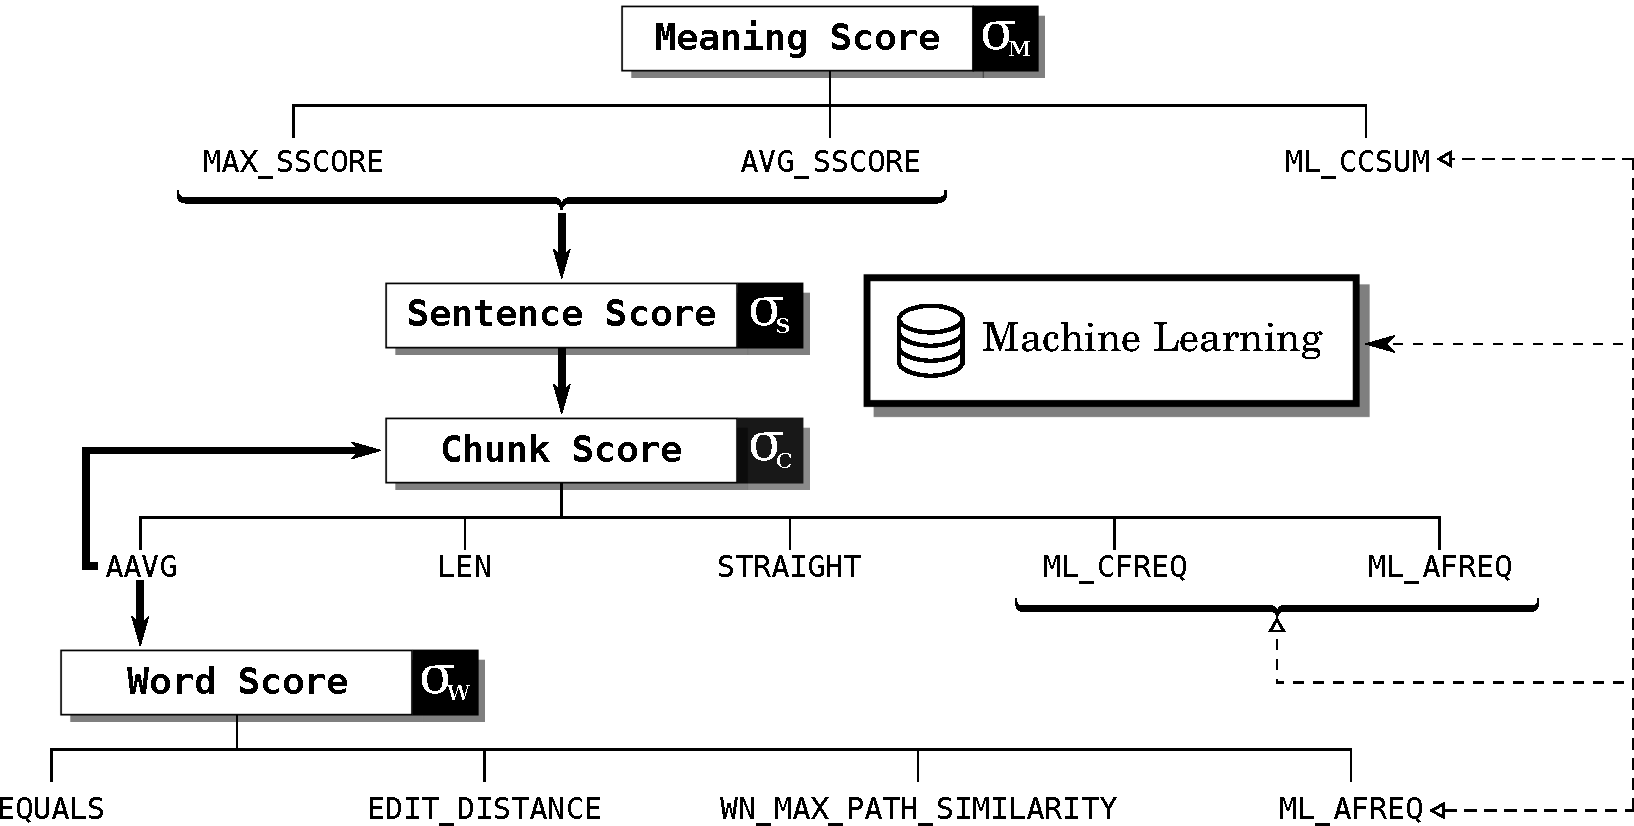
\includegraphics[width=23cm]{Pictures/scores_diagram.pdf}
\caption{Scores' structure}
\label{scoresbreakdown}
\end{sidewaysfigure}